
  \begin{figure}[ht!]

    \noindent\makebox[\textwidth]{%
    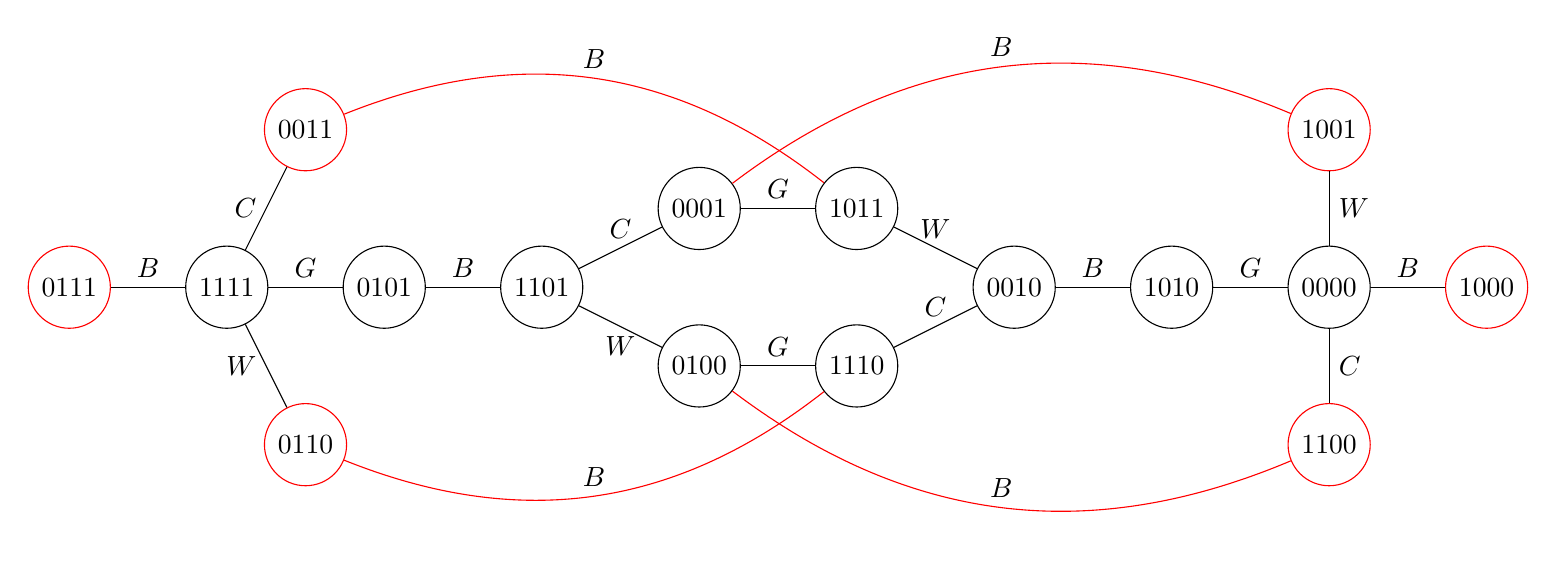
\begin{tikzpicture}[block/.style={circle}]
    \node[shape=circle, draw=black] (0000) at (9,0) {0000};
    \node[shape=circle, draw=black] (0001) at (1,1) {0001};
    \node[shape=circle, draw=black] (0010) at (5,0) {0010};
    \node[shape=circle, draw=red] (0011) at (-4,2) {0011};
    \node[shape=circle, draw=black] (0100) at (1,-1) {0100};
    \node[shape=circle, draw=red] (0110) at (-4,-2) {0110};
    \node[shape=circle, draw=red] (0111) at (-7, 0) {0111};
    \node[shape=circle, draw=red] (1000) at (11,0) {1000};
    \node[shape=circle, draw=red] (1001) at (9,2) {1001};
    \node[shape=circle, draw=black] (1010) at (7,0) {1010};
    \node[shape=circle, draw=black] (1011) at (3,1) {1011};
    \node[shape=circle, draw=red] (1100) at (9,-2) {1100};
    \node[shape=circle, draw=black] (1110) at (3,-1) {1110};
    \node[shape=circle, draw=black] (1111) at (-5,0) {1111};
    \node[shape=circle, draw=black] (0101) at (-3,0) {0101};
    \node[shape=circle, draw=black] (1101) at (-1,0) {1101};

    \path [-] (1111) edge node[above] {$G$} (0101);
    \path [-] (1111) edge node[above] {$B$} (0111);
    \path [-] (1111) edge node[left] {$C$} (0011);
    \path [-] (1111) edge node[left] {$W$} (0110);

    \path [-] (0101) edge node[above] {$B$} (1101);

    \path [-] (1101) edge node[above] {$C$} (0001);
    \path [-] (1101) edge node[below] {$W$} (0100);

    \path [-] (0001) edge node[above] {$G$} (1011);
    \path [-] (0100) edge node[above] {$G$} (1110);

    \path [-] (1011) edge node[above] {$W$} (0010);
    \path [-] (1110) edge node[above] {$C$} (0010);

    \path [-] (0010) edge node[above] {$B$} (1010);

    \path [-] (1010) edge node[above] {$G$} (0000);

    \path [-] (0000) edge node[right] {$W$} (1001);
    \path [-] (0000) edge node[above] {$B$} (1000);
    \path [-] (0000) edge node[right] {$C$} (1100);

    \path [-] (0011) edge[bend left,draw=red] node[above] {$B$} (1011);
    \path [-] (0110) edge[bend right,draw=red] node[above] {$B$} (1110);

    \path [-] (1001) edge[bend right,draw=red] node[above] {$B$} (0001);
    \path [-] (1100) edge[bend left,draw=red] node[above] {$B$} (0100);

    \end{tikzpicture}
    }
    \caption{Graph with error states and transitions.}
  \end{figure}

  \begin{figure}[ht!]

      \noindent\makebox[\textwidth]{%
      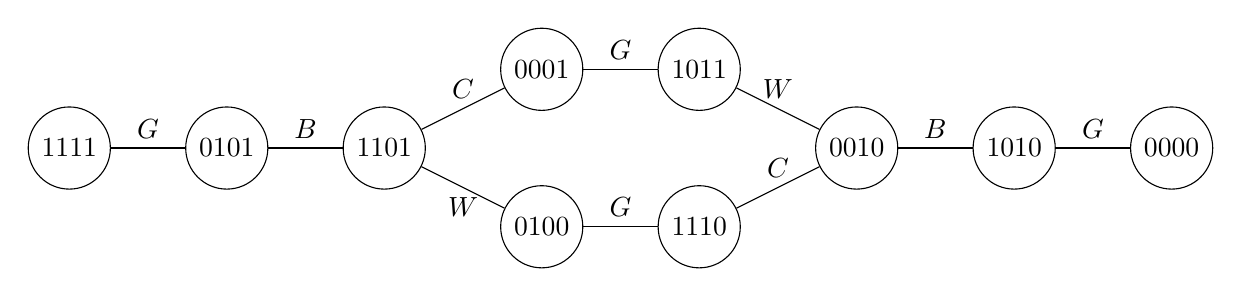
\begin{tikzpicture}[block/.style={circle}]
      \node[shape=circle, draw=black] (0000) at (9,0) {0000};
      \node[shape=circle, draw=black] (0001) at (1,1) {0001};
      \node[shape=circle, draw=black] (0010) at (5,0) {0010};
      \node[shape=circle, draw=black] (0100) at (1,-1) {0100};
      \node[shape=circle, draw=black] (1010) at (7,0) {1010};
      \node[shape=circle, draw=black] (1011) at (3,1) {1011};
      \node[shape=circle, draw=black] (1110) at (3,-1) {1110};
      \node[shape=circle, draw=black] (1111) at (-5,0) {1111};
      \node[shape=circle, draw=black] (0101) at (-3,0) {0101};
      \node[shape=circle, draw=black] (1101) at (-1,0) {1101};

      \path [-] (1111) edge node[above] {$G$} (0101);
      \path [-] (0101) edge node[above] {$B$} (1101);
      \path [-] (1101) edge node[above] {$C$} (0001);
      \path [-] (1101) edge node[below] {$W$} (0100);
      \path [-] (0001) edge node[above] {$G$} (1011);
      \path [-] (0100) edge node[above] {$G$} (1110);
      \path [-] (1011) edge node[above] {$W$} (0010);
      \path [-] (1110) edge node[above] {$C$} (0010);
      \path [-] (0010) edge node[above] {$B$} (1010);
      \path [-] (1010) edge node[above] {$G$} (0000);

      \end{tikzpicture}
      }
      \caption{Graph without error states.}
      \end{figure}
